% ========== GRÅAND ==========
\begin{frame}{%
  \begin{minipage}[t]{0.32\textwidth}
    Gråand
  \end{minipage}%
  \hfill
  \begin{minipage}[t]{0.36\textwidth}
    \centering
    \footnotesize\textbf{Jagttid:} 1.\ september -- 31.\ januar
  \end{minipage}%
  \hfill
  \begin{minipage}[t]{0.15\textwidth}
    \noindent\raggedleft
    
\includegraphics[width=0.5cm, height=0.5cm, keepaspectratio]{Billeder/Ikoner/star.png}%
    \hspace{0.2em}%
    
\includegraphics[width=0.5cm, height=0.5cm, keepaspectratio]{Billeder/Ikoner/star.png}%
    \hspace{0.2em}%
    
\includegraphics[width=0.5cm, height=0.5cm, keepaspectratio]{Billeder/Ikoner/star.png}
  \end{minipage}%
}
  \vspace{0.25em}
  \begin{columns}[T]
    % --- Venstre kolonne: Tekst ---
    \column{0.55\textwidth}
    \setlength{\parskip}{0.5em}
    \tiny
    \RaggedRight
    \textbf{\textit{Anas platyrhynchos}} – stor svømmeand med rappende kald, også kaldet vildand, moseand, stokand \par
    \textbf{Udseende:}\\
    \quad – Andrik: Hvid halsring, metalblåt vingespejl \par
    \quad – And: Gulligt næb, blåt vingespejl \par
    \textbf{Levesteder:} Søer, moser, fjorde og vandløb. \par
    \textbf{Føde:} Dyre- og planteføde, herunder hvede og byg. \par
    \textbf{Udbredelse:} Hele Danmark. \par
    \textbf{Træk/standfugl:} Begge (trækfuglene kommer efter oktober)
    \begin{itemize}
      \itemsep0pt
      \item \textbf{Yngleforhold:} Yngler i hele Danmark.
      \item \textbf{Kønsmoden:} Ca. 1 år
      \item \textbf{Mono/polygam:} Monogam
      \item \textbf{Bestandsomsætning:} Hurtig
      \item \textbf{Kuld:} 9–13 æg
      \item \textbf{Jagttid:} 1.\ september -- 31.\ januar
    \end{itemize}
    % --- Højre kolonne: Billeder ---
    \column{0.40\textwidth}
    \centering
    \fbox{%
      \begin{minipage}{\linewidth}
        \centering
        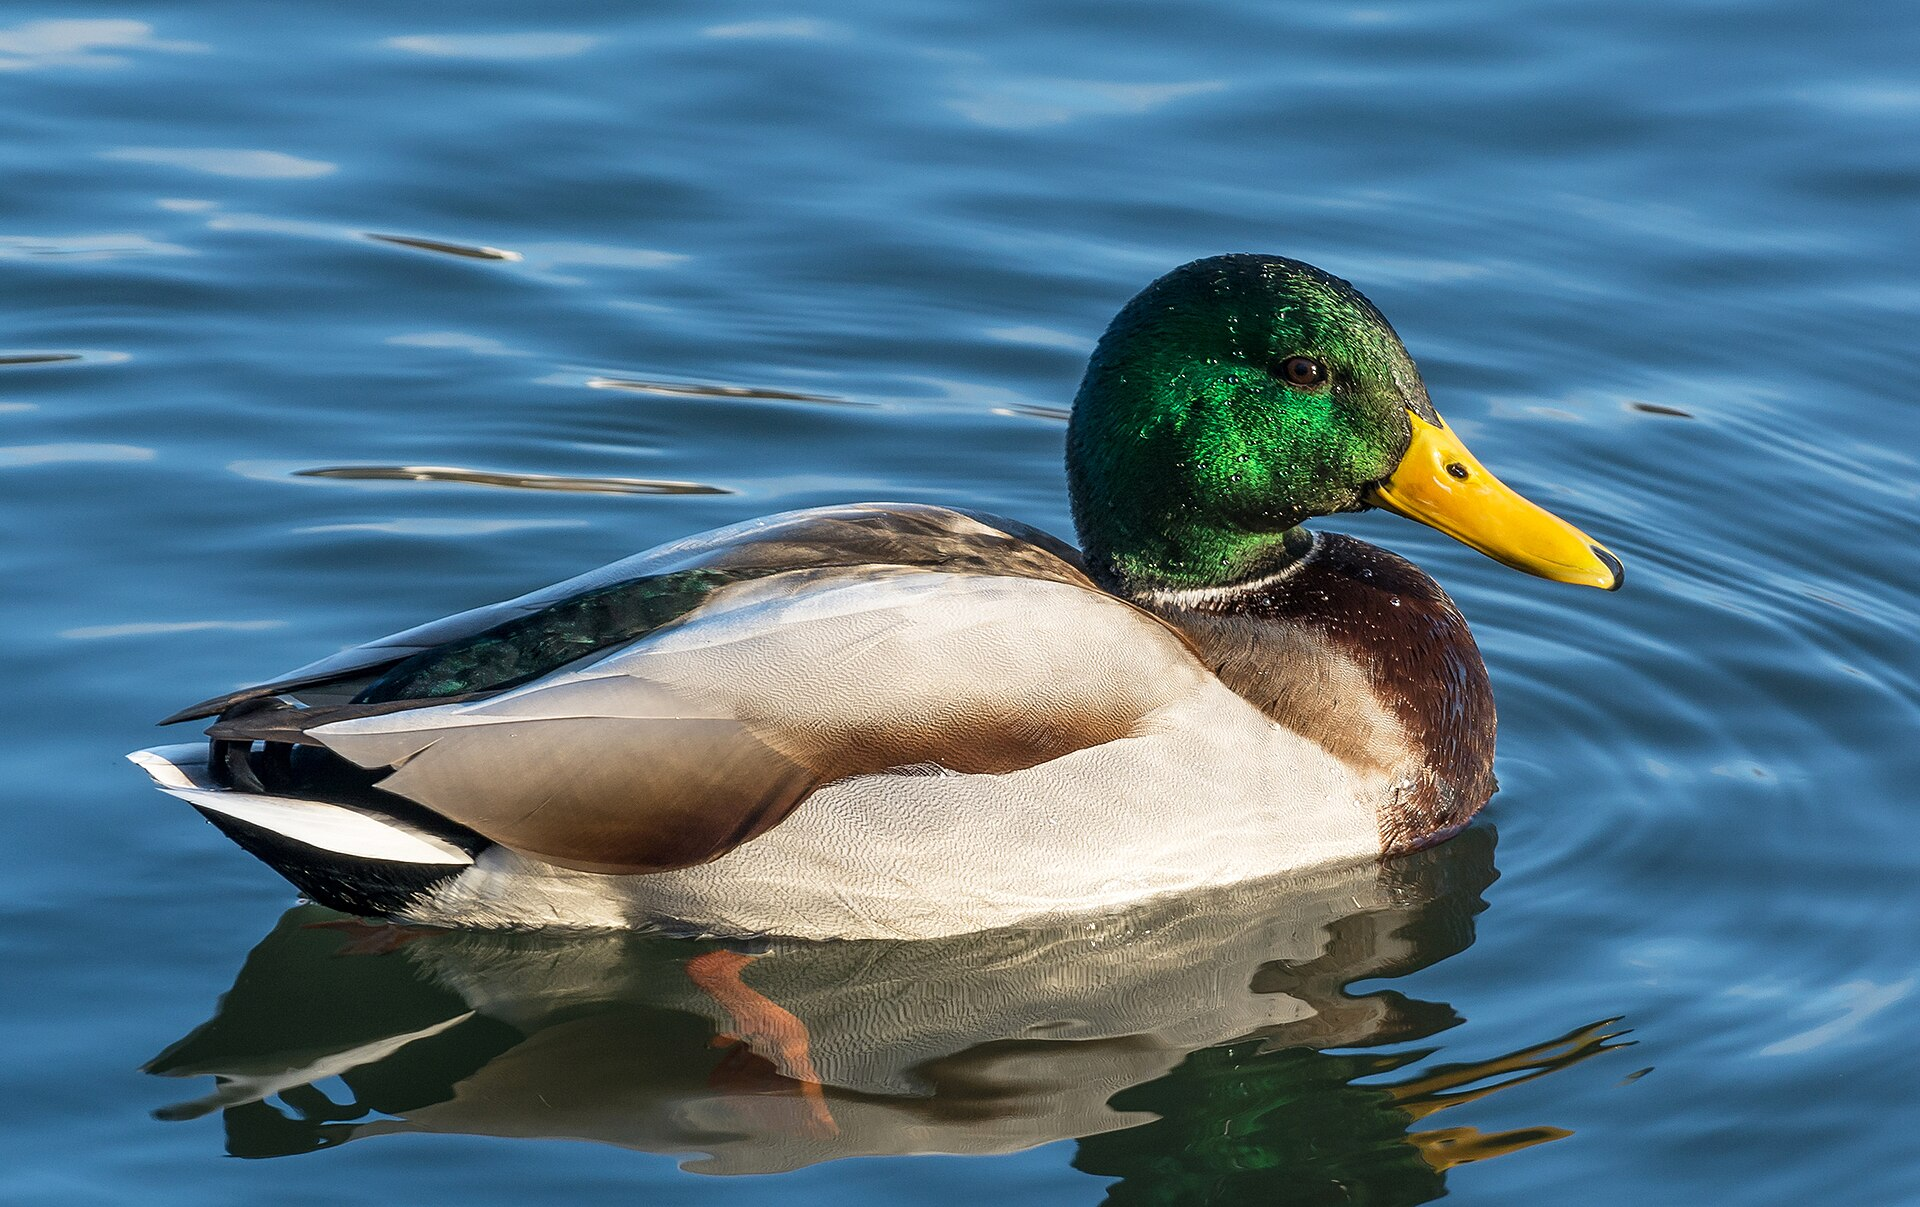
\includegraphics[width=0.7\linewidth, height=3cm, keepaspectratio]{Billeder/Dyr/Fugle/Aender/Svoemmeaender/gråand_han.jpg}\\[0.5em]
        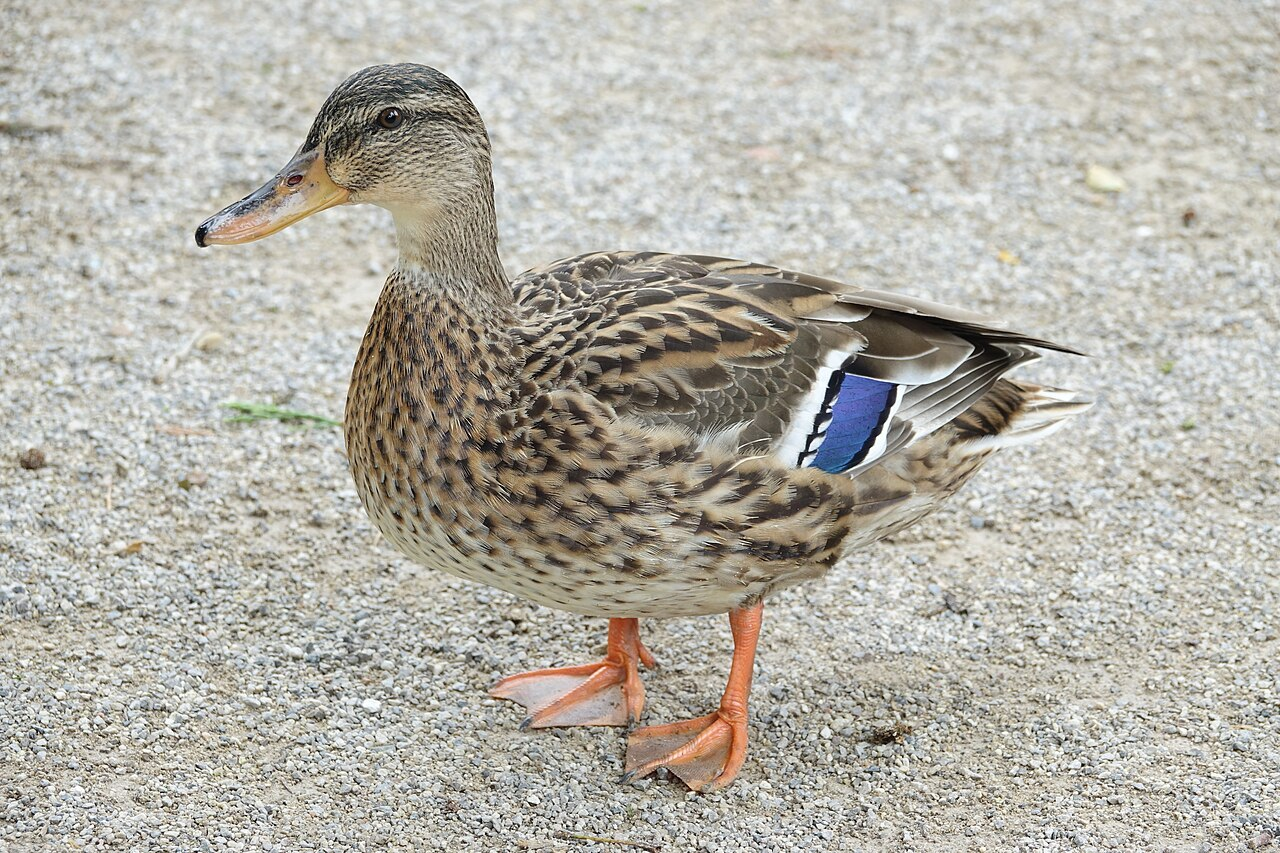
\includegraphics[width=0.7\linewidth, height=3cm, keepaspectratio]{Billeder/Dyr/Fugle/Aender/Svoemmeaender/gråand_hun.jpg}%
      \end{minipage}
    }%
    \vspace{0.05em}
    \footnotesize Andrik øverst, and nederst
  \end{columns}
\end{frame}